\documentclass{cernatsnote}
\usepackage{siunitx}
\usepackage[table,xcdraw]{xcolor}
\usepackage{soul}
%\usepackage[colorinlistoftodos]{todonotes}
\usepackage{placeins}
\usepackage{titlesec}
\usepackage{subfigure}
\usepackage{float}
\usepackage{booktabs}
\setcounter{secnumdepth}{4}
\setcounter{tocdepth}{4}    %
\usepackage{amssymb}
\usepackage{url}

\usepackage{booktabs}
\usepackage{multirow}
\usepackage{rotating,tabularx}
\usepackage{tikz}
\usetikzlibrary{patterns}
\usepackage{array}

\usepackage{multirow}
\usepackage{graphicx}
\usepackage{threeparttable}

\title{ESA Technical note on on solution implemented for the primary beam energy reduction}
\author{
	E. Johnson, P.A. Arrutia Sota, K. Bilko, M. Delrieux, N. Emriskova,\\ A. Waets, A. Coronetti,  M.A. Fraser, R. Garcia Alia\; \\		
	CERN, CH-1211 Geneva, Switzerland
}
\emailb{ruben.garcia.alia@cern.ch}
\emaila{eliott.philippe.johnson@cern.ch}
\date{\today}

\setlength {\marginparwidth }{2cm}
\begin{document}
\maketitle

\begin{abstract}
This technical note describes a solution implemented for the primary beam energy adjustment for the heavy ion irradiation activities in the CHARM facility project at CERN. The beam energy was varied by scaling the magnetic field in the Proton Synchrotron (PS) during acceleration and transport. The PS's magnet strengths were adjusted by an algorithm (makerule) that computes the magnetic field required for a given beam energy, allowing automatic scaling of magnets in F61 and the T8 transfer line. This note presents the results of the beam energy measurements during the November 2022 run and discusses the limitations of the system.

\end{abstract}
\\ \\ \\ 

\newpage

\sethlcolor{yellow}
\begin{table}[!htp]
\centering
{\tiny
\begin{tabular}{@{}p{2.5cm}p{2cm}p{2cm}p{2.4cm}p{5cm}@{}}
\toprule
Contract name & Contract number - ESA & Contract number - CERN & Task & Technical Note or Report \\
\midrule
Development of High Energy Beam (range and LET) for Radiation Tests of Highly Integrated Electronics components &
4000134554\linebreak/21/NL/KML/rk &
KM5174\linebreak/KT/SY/273A &
Task 1: CERN CHARM ion beam energy reduction &
\hl{TN1: Technical note on solution implemented for the primary beam energy reduction}\\
&  &  & Task 2: Beam calibration and dosimetry & TR1: Test Report with calibration and dosimetry measurements\\
 &  &  &  & TN2: Technical Note on the dosimetry methodologies and procedures for calibration and routine beam operations\\
High Energy Beam Intensity Adjustment for SEE tests of COTS EEE Components & 4000136601\linebreak/21/NL/KML/rk & KM5450\linebreak/KT/SY/276R & Task 1: Primary beam intensity adjustments & TN1: Technical Note on solution implemented for the flux adjustments\\
 &  &  & Task 2: Beam calibration and dosimetry & TR1: Test report with initial and final results of calibration and dosimetry measurements, example of test report that will be provided for routine operation\\
 &  &  & Task 3: Preparation of test execution process for industry & TN2: Technical note. Guideline for test users: with necessary information for external users to prepare and execute a test at the facility\\
 &  &  &  & TR2: Test report of SEE tests\\
 \bottomrule
\end{tabular}
}
\end{table}

\newpage

\begingroup
\color{black}
\tableofcontents
\endgroup

\pagebreak

\section{Introduction}
In the field of radiation testing of electronic components, controlling the primary beam energy is a critical aspect of ensuring accurate and reliable results. For a given particle species, the primary beam energy determines the Linear Energy Transfer (LET), a measure of the energy deposited by a particle as it travels through a material, which in turn affects the type and amount of radiation-induced effects on the electronic components being tested. By varying the primary beam energy, different ranges of LET are available to study the effects of radiation at different levels of energy deposition, which is important for understanding how electronic components will behave in different radiation environments. For example, in space applications, electronic components are exposed to high-energy particles with a wide range of LET values, and it is essential to understand how these particles will affect the performance and reliability of the components. Therefore, the ability to control the primary beam energy and explore different LET values is critical for accurately characterizing the radiation response of electronic components and designing robust systems for space and other radiation environments.

This technical note detailing the solution implemented for primary beam energy variation is an important milestone to providing a heavy ion irradiation program at CERN because it provides a method for controlling primary beam energy and exploring a wide range of LET values. The variation of the primary beam energy was achieved by scaling the magnetic field in the Proton Synchrotron (PS) during acceleration by adjusting the PS's magnet strengths according to a makerule that computed the magnetic field required for a given beam energy. The makerule also allows for the automatic scaling of magnets in F61 and the T8 transfer line, which are required to transport the heavy ion beam to CHARM. The note details the various steps taken during the run, including characterization of the three beam energies, testing of the four Device Under Test (DUT) setups, and a degrader scan. Furthermore, the note presents the results of the beam energy measurements during the November 2022 run and discusses the limitations of the system.

\begin{figure}[!htb]
\centering
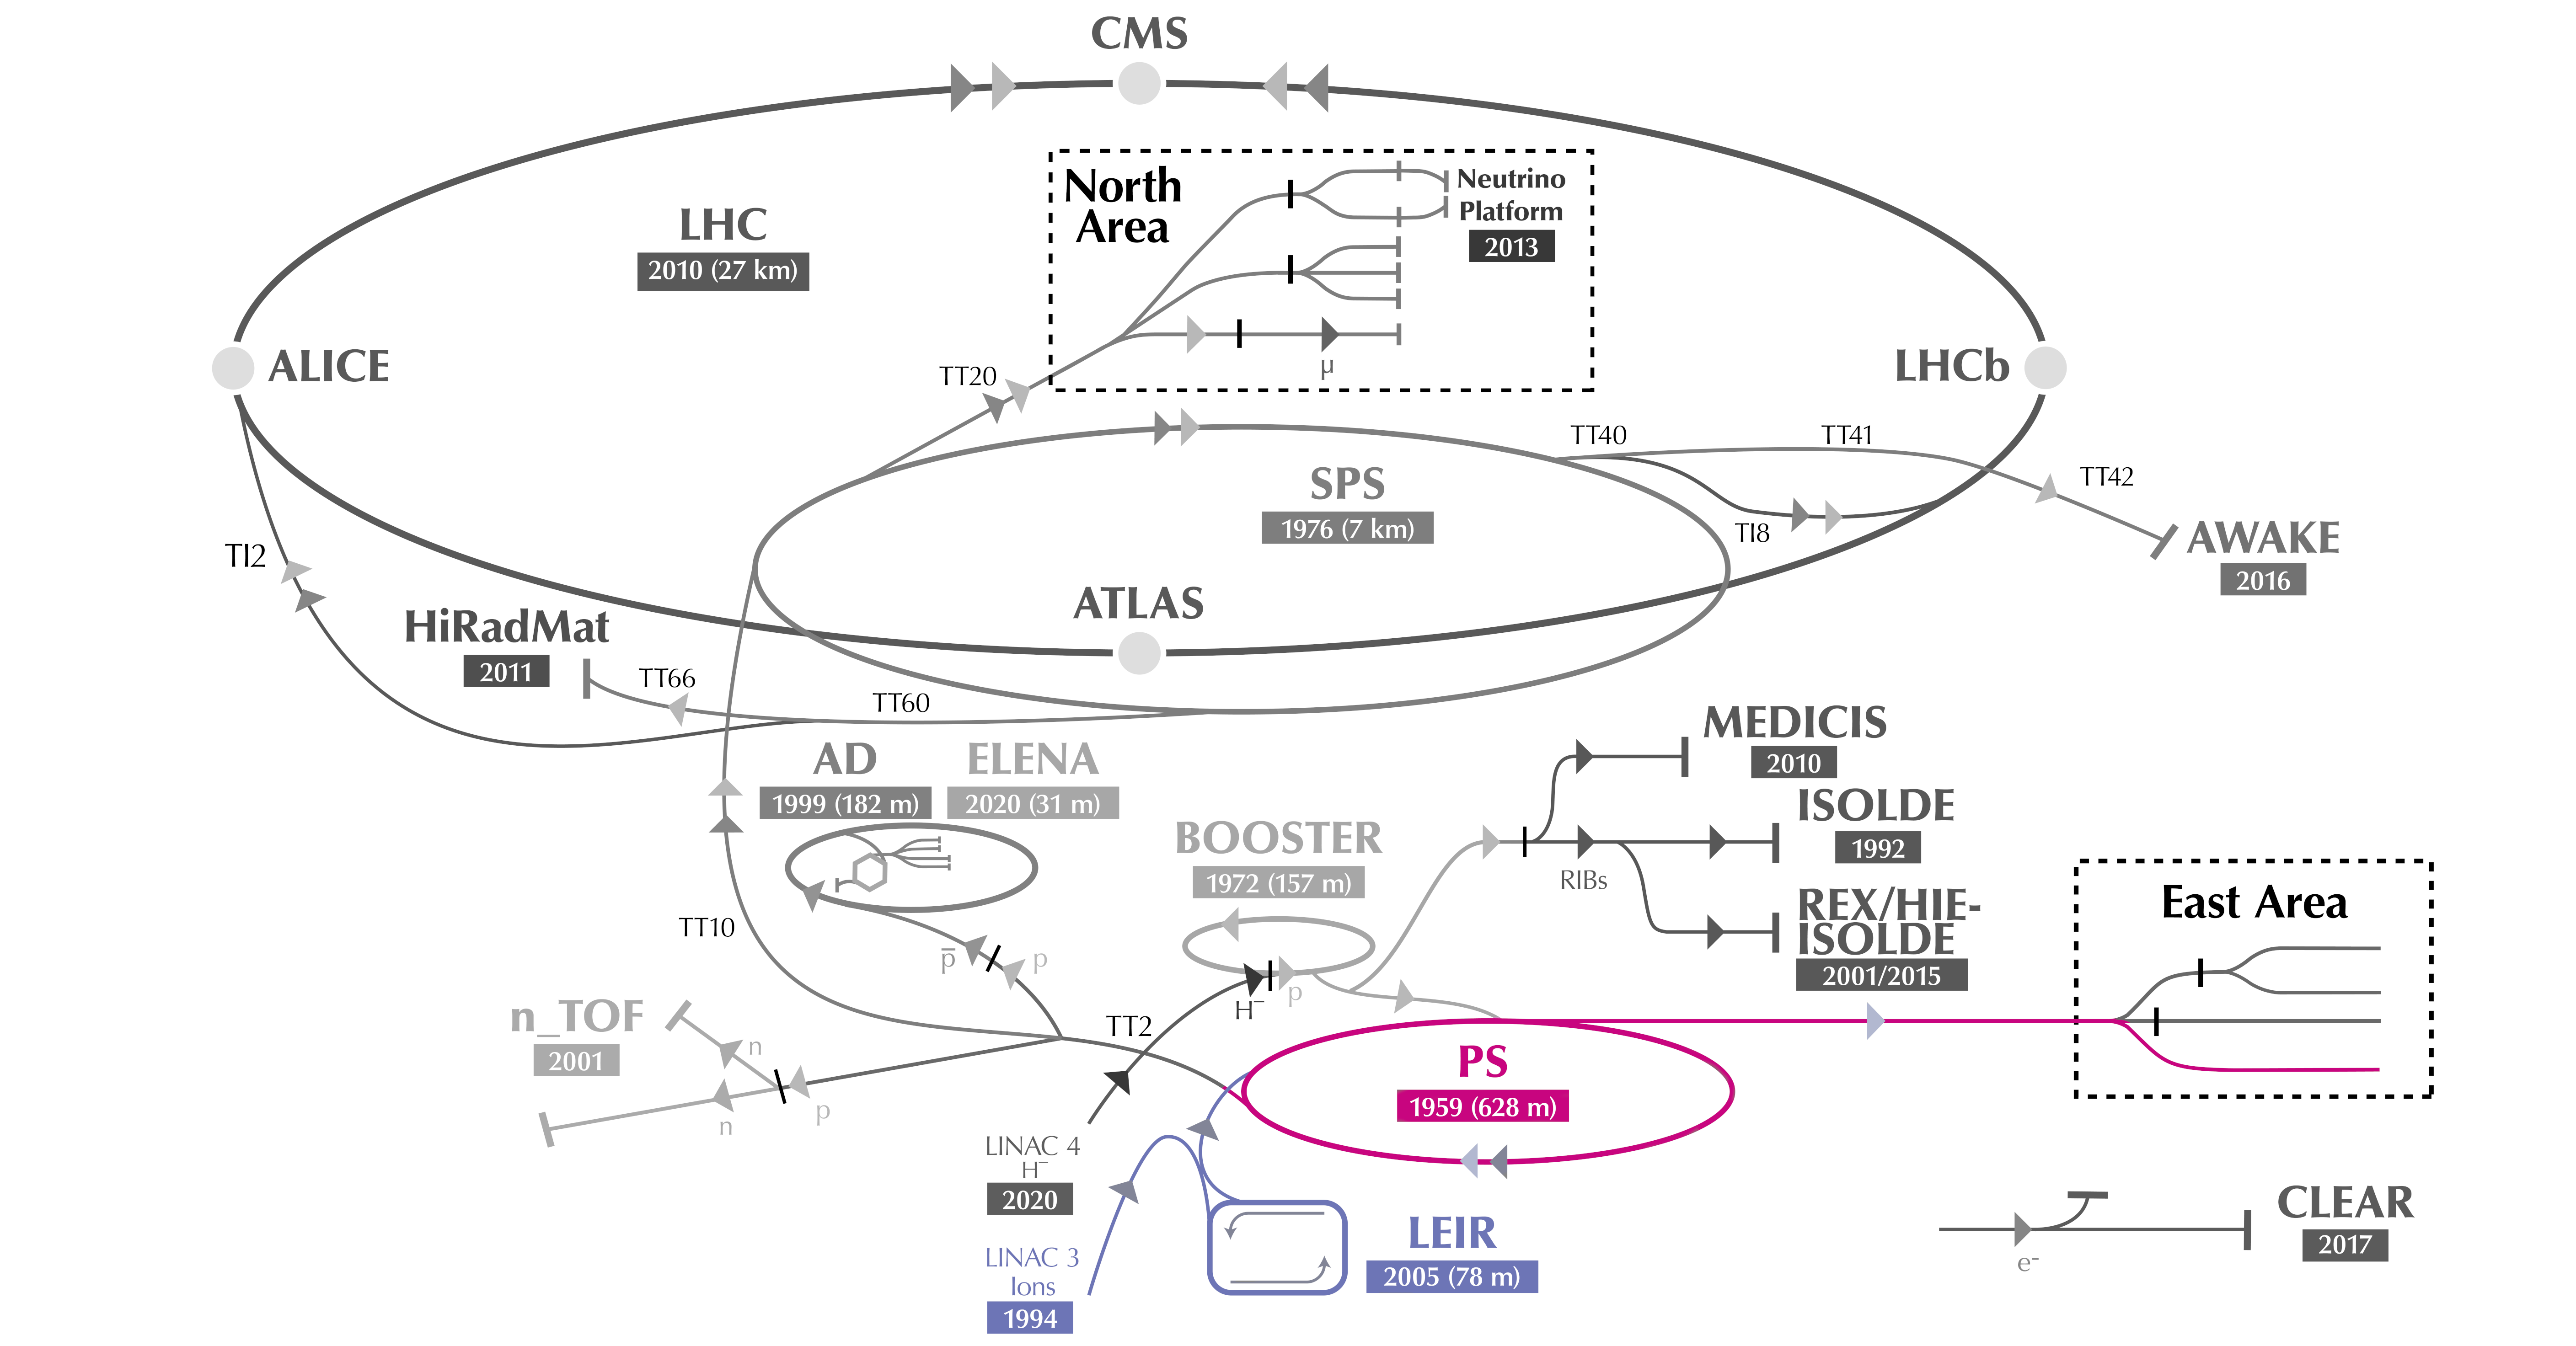
\includegraphics[width=1.0\textwidth]{images/CCC_eastt8_small.png}
\caption{The CERN accelerator complex. The path of the lead ion beam used for the ion irradiation activity in CHARM is highlighted in color.}
\label{fig:CCC}
\end{figure}


\section{Energy variation}

The Proton Synchrotron (PS) is a crucial component of the accelerator complex, responsible for accelerating particles from the Proton Synchrotron Booster (PSB) to the Super Proton Synchrotron (SPS) and ultimately to the Large Hadron Collider (LHC). Additionally, the PS is capable of receiving and accelerating heavy ions from the Low Energy Ion Ring (LEIR) for extraction to the East Area, making it a versatile machine. RF cavities are used to accelerate charged particles, such as protons or lead ions, to high energies, while 100 dipoles bend the beam around the PS's 628 m circumference \cite{gilardoni_fifty_2011}. The particles are then extracted using slow extraction through a beam line and transported to the CHARM facility, which houses the beam instruments and irradiation setups. .
\\

The beam energy refers to the kinetic energy per nucleon $E_{kin}$ of the charged particle beam. For an ion beam, the total kinetic energy, denoted $E_{kin, TOT}$, can be obtained by multiplying $E_{kin}$ by the atomic mass number $A$ (where $A = Z + N$, representing the total number of protons $Z$ and neutrons $N$ in the nucleus). The total momentum for an ion beam is given by \cite{chao_handbook_2013}

$$pc={E_{0}\sqrt{\gamma^{2}-1}}$$

$$pc = E_{0}\sqrt{\left [ \left( \frac{E_{kin, TOT}}{E_{0}}+1\right )^{2}-1\right ]}$$
where, $E_{0}$ is the rest mass of the ion and $\gamma=\frac{E}{E_{0}}=\frac{E_{0}+E_{kin}}{E_{0}} = \frac{E_{kin}}{E_{0}}+1$
\\

The ion irradiation activity in CHARM (CHIMERA) uses a lead ion beam. In the PS the beam is a partially stripped ion beam of Pb$^{54+}$, which means that 28 $e^{-}$ remain on the ion for the isotope A=208.
\\

\begin{figure}
    \centering
    \begin{minipage}{0.45\textwidth}
        \centering
        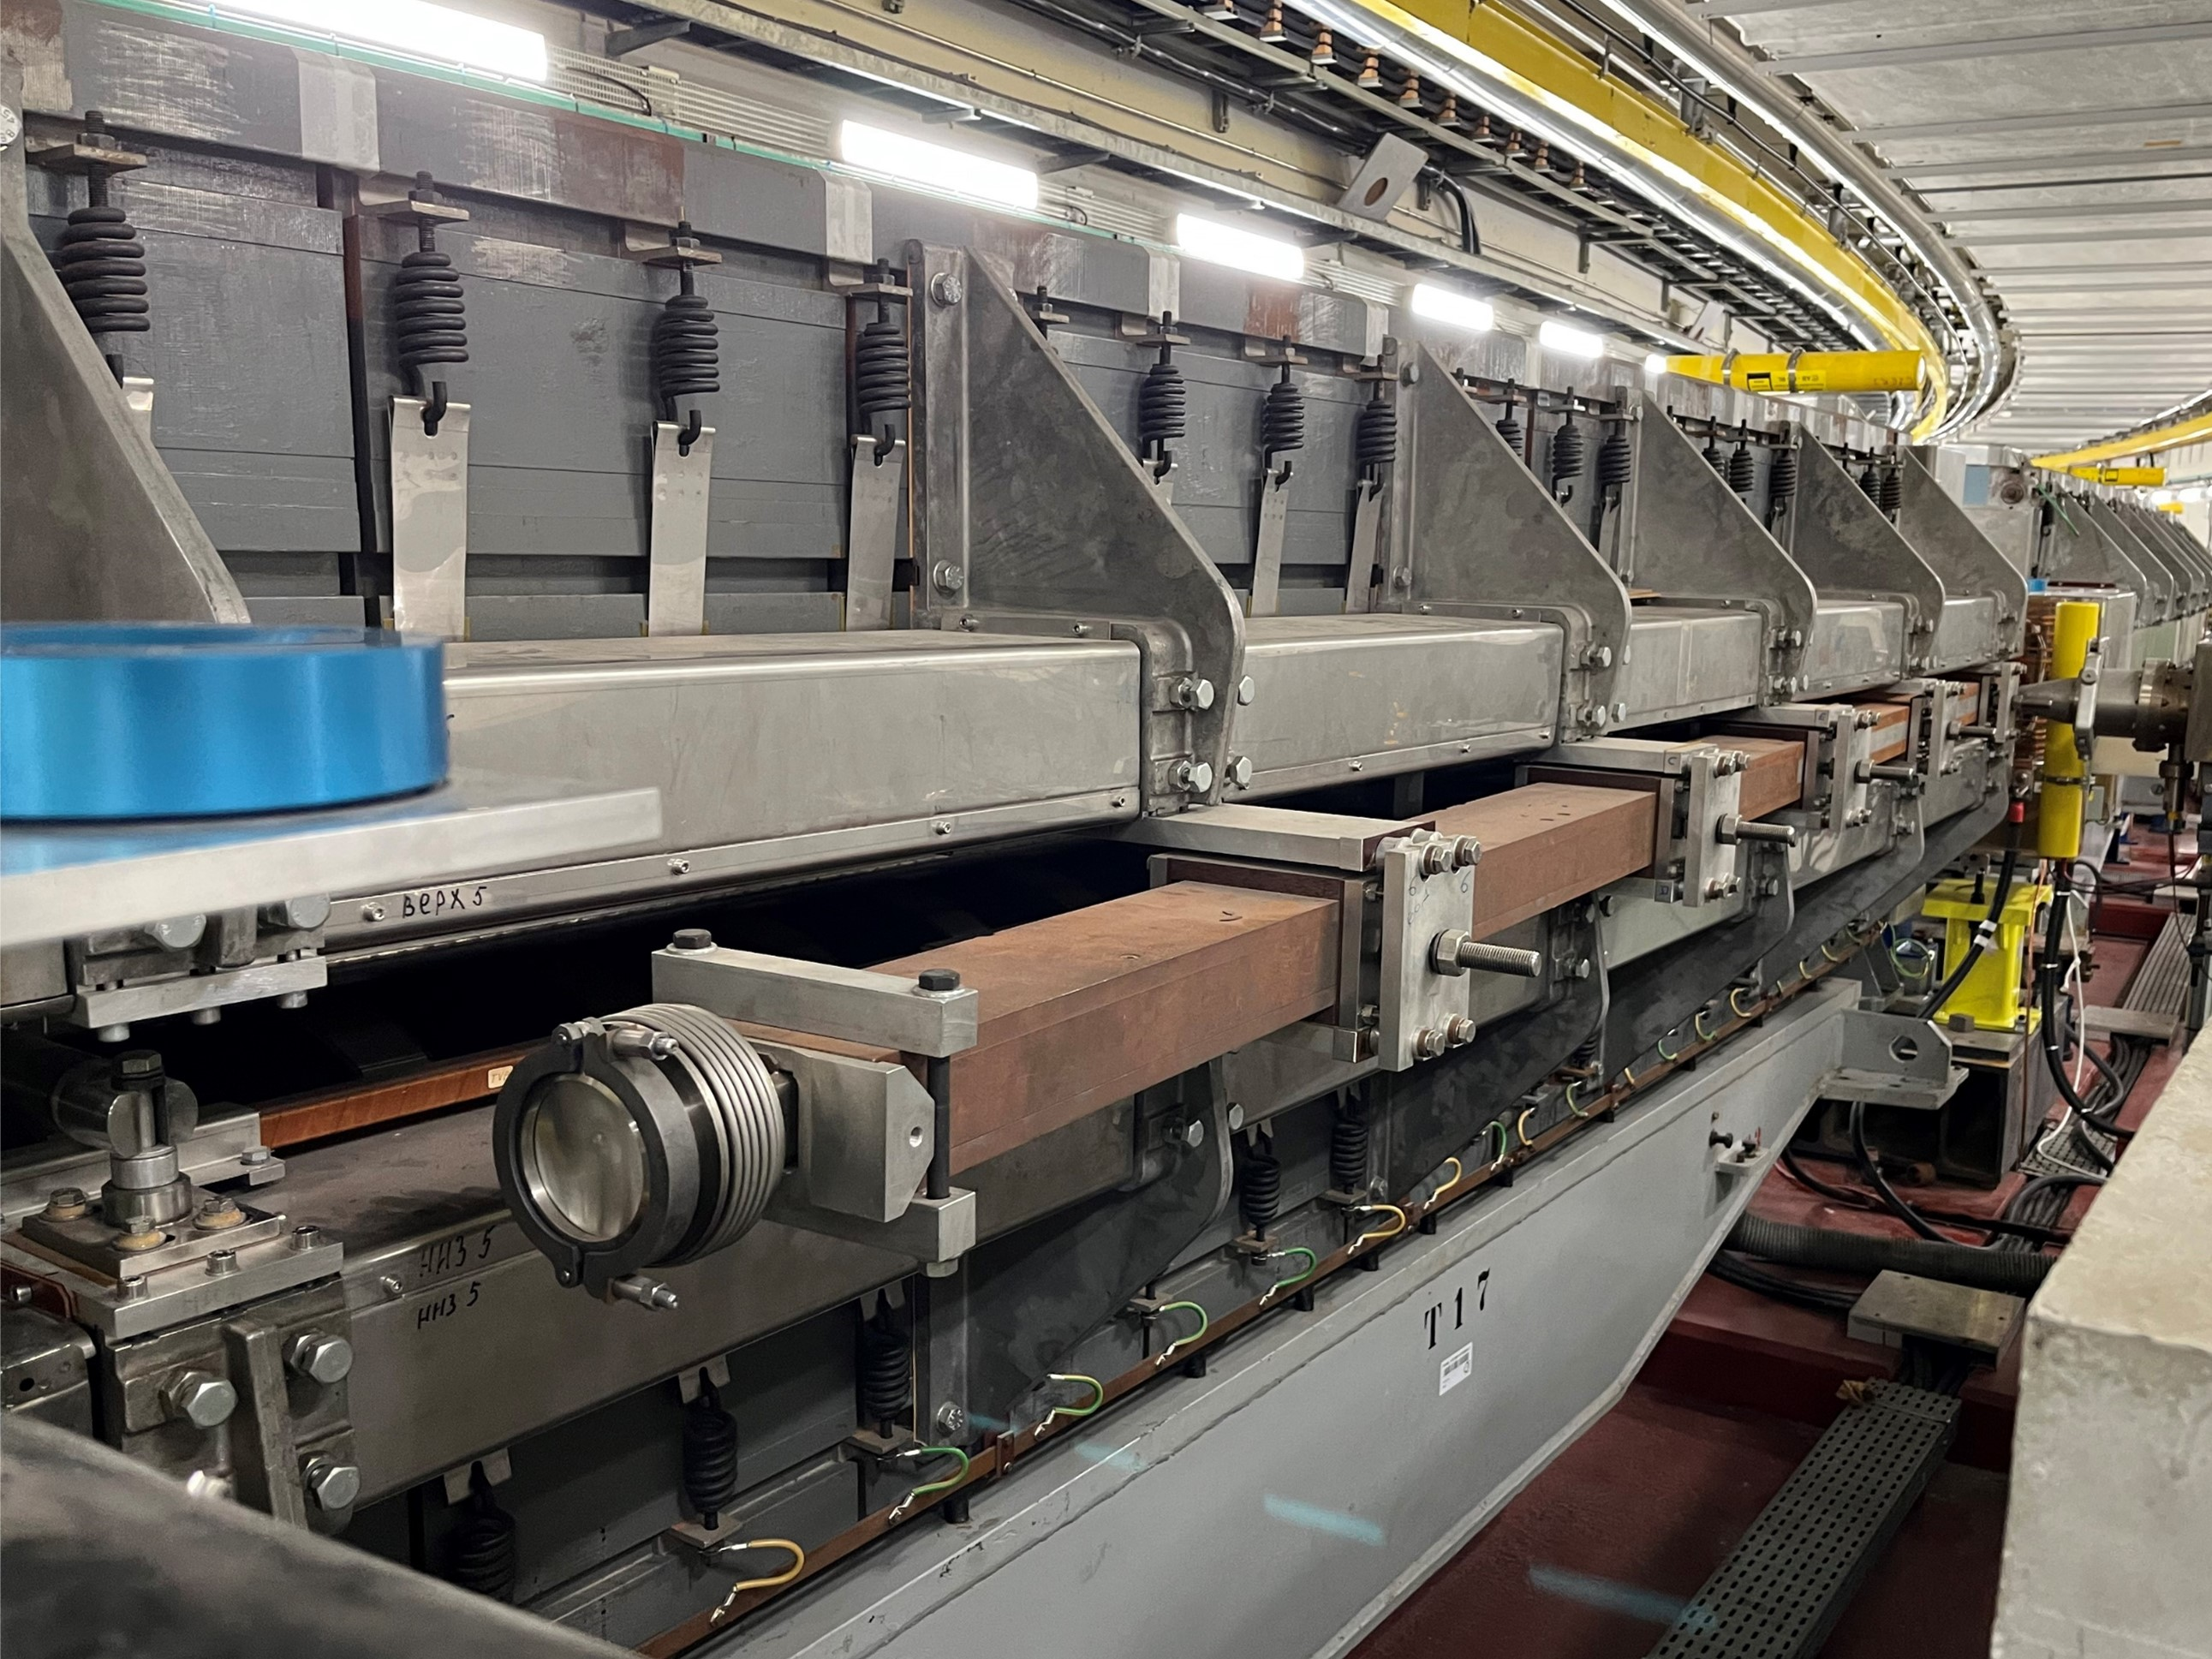
\includegraphics[width=1.0\textwidth]{images/PS_BEAM_ENERGY/vaccum_window.jpg}
        \caption{Vacuum window connecting the PS to the transfer line leading to the East Area.}
        \label{fig:vaccum window}
    \end{minipage}\hfill
    \begin{minipage}{0.45\textwidth}
        \centering
        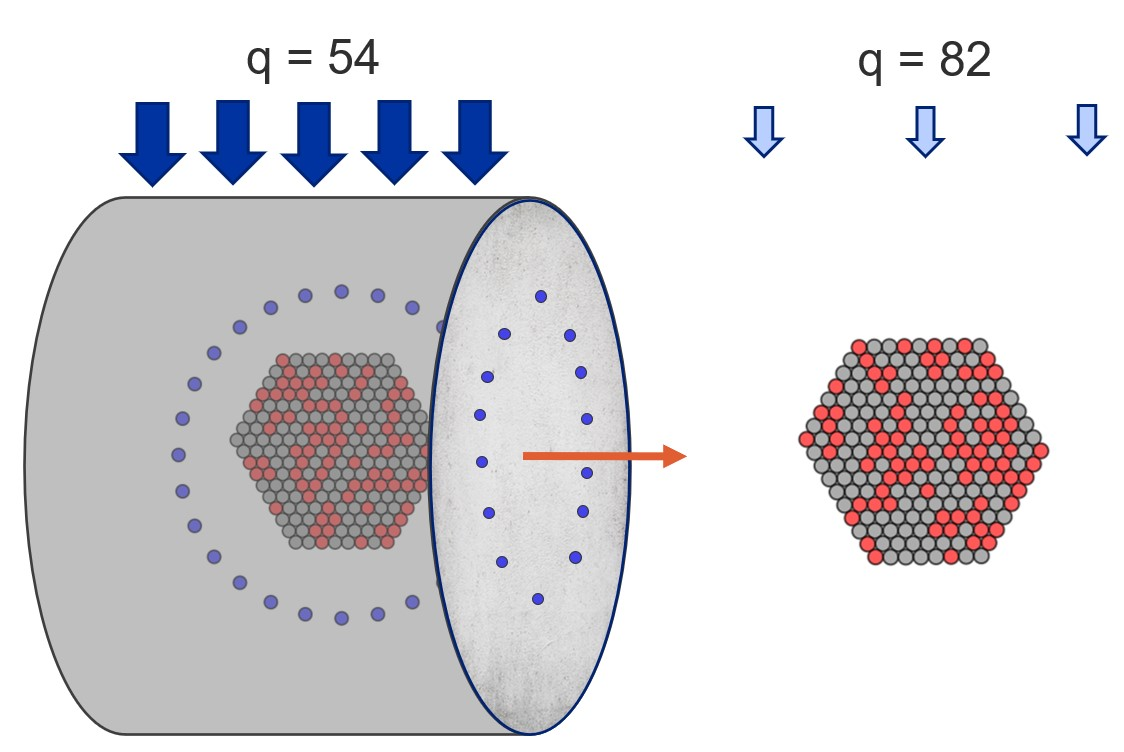
\includegraphics[width=1.0\textwidth]{images/PS_BEAM_ENERGY/stripping.jpg} 
        \caption{Diagram illustrating the stripping process, where an ion loses its remaining electrons. The resulting ion has a higher charge state when it travels through the transfer line.}
        \label{fig:stripping}
    \end{minipage}
\end{figure}

As an example, for a kinetic energy of 1 GeV/$u$ (per nucleon) the total momentum would be:

$$p = E_{0}\sqrt{\left [ \left( \frac{1\text{ [GeV]}\cdot 208}{E_{0}}+1\right )^{2}-1\right ]} = 351.9 \left[\frac{\text{GeV}}{\text{c}}\right]$$
where the rest mass $E_{0}$ of Pb$^{54+}$ is:

$$E_{0} = m_{Pb54+}= 82\cdot m_{proton} + 126\cdot m_{neutron} + 28\cdot m_{e^{-}} - m_{defect} = 193.74 \left[\frac{\text{GeV}}{\text{c}^{2}}\right]$$
with mass defect; see Table \ref{table:masses}: $m_{defect}=82\cdot m_{proton} + 126\cdot m_{neutron} + 28\cdot m_{e^{-}} - 208\cdot m_{u}$ 

\begin{table}[h!]
\centering
\begin{tabular}{lr}
\toprule
Particle & mass GeV/$\text{c}^{2}$\\
\midrule
$m_{proton}$ & 0.93828      \\
$m_{neutron}$ & 0.93957      \\
$m_{e^{-}}$ & 0.000511 \\
$m_{u}$ & 0.9315       \\
\bottomrule
\end{tabular}
\caption{Rest masses \cite{boston_university_nuclear_nodate}.}
\label{table:masses}
\end{table}

The beam momentum is related to the magnetic rigidity [Tesla meter] as follows: 
$$B\rho \text{ [T m]} = 3.3356\cdot p/q \text{ [GeV/c]}$$
where for the PS, $\rho = 70.0789$ m. This formula is used to calculate the bending B-field in the PS dipoles.
\\

For the 2022 CHIMERA run, three primary kinetic energies at flat-top in the PS were selected: 1000, 750, and 650 MeV/$u$, and the associated required magnetic fields (B-fields) were calculated, as shown in Fig. \ref{fig:lookup table} and Table \ref{tab:KE_table}. However, interaction with vacuum windows, instruments, and air molecules during transport through the transfer line lowers the beam's kinetic energy. Therefore, a FLUKA model simulation is required to determine the beam energy at the Device Under Test (DUT) in CHARM. The FLUKA simulation model includes rigidities for each of the primary energies, along with an accurate representation of the material budget that the beam crosses when transported through the transfer line, which includes all vacuum windows, beam instrumentation, and air regions. The simulations reveal that the compound effect of all the materials in the beam causes energy straggling, resulting in significantly lower beam kinetic energies at the DUT position. Table \ref{tab:KE_table} presents the primary kinetic energy degradation from the PS to the DUT. Consequently, the range of beam LETs that can be obtained by varying the beam energy is larger, which is one of the fundamental radiation effects testing metrics. The simulations show that by varying the primary beam energy extracted from the PS, the resulting LET at the DUT can vary between 10 and 30 MeVcm$^2$/mg. When additional dedicated sheets of material, such as PPMA, are placed in the beam, it is possible to achieve LETs greater than 30 MeVcm$^2$/mg.
\\

Significant effort has been invested in automating the scaling of magnets in F61 and the T8 transfer line to reduce the operational overhead of operating the irradiation facility at different beam energies. The removal from operation of the Pole Face Windings (PFW) in the PS was necessary to allow for continuous energy variation as they do not scale with beam rigidity in a linear way. The T8 transfer line has been converted to Pulse to Pulse Modulation (PPM), which means that the magnet strengths are user-based and different users (or energies) can be sent to the East Area in parallel. This enable the use of different beams during the same super-cycle, whereas in non-PPM mode, only a single user or type of beam could be used. A makerule is used to compute the correct strength to apply based on the PS B-field (and thus beam energy).
\\

Moreover, since the ion beam is partially stripped in the PS and becomes fully stripped after passing through the exit vacuum window in the F61 transfer line, located after the first quadrupole in the transfer line (Q74L), different rigidities are required for acceleration and transport, respectively. Therefore, the magnets in the transfer line must be pulsed with a rigidity matched to the fully stripped ion beam. The makerule computes a partially stripped momentum for the first quadrupole in F61 and a second momentum for a fully stripped ion beam for the rest of the transfer line down to CHARM. This automatic scaling is highly advantageous, as energy scans can be performed by merely adjusting the B-field at the flat-top of the PS.
\\

However, there are some limitations to this automatic scaling process. For example, the extraction path often requires occasional manual corrections, which involves adjusting the strength of the septum magnets used for extraction, namely SMH57 and SMH61. Additionally, the bending to the East Dump can not be associated with a makerule, and only a scalar current can be set.
\\

\begin{figure}[!htb]
\centering
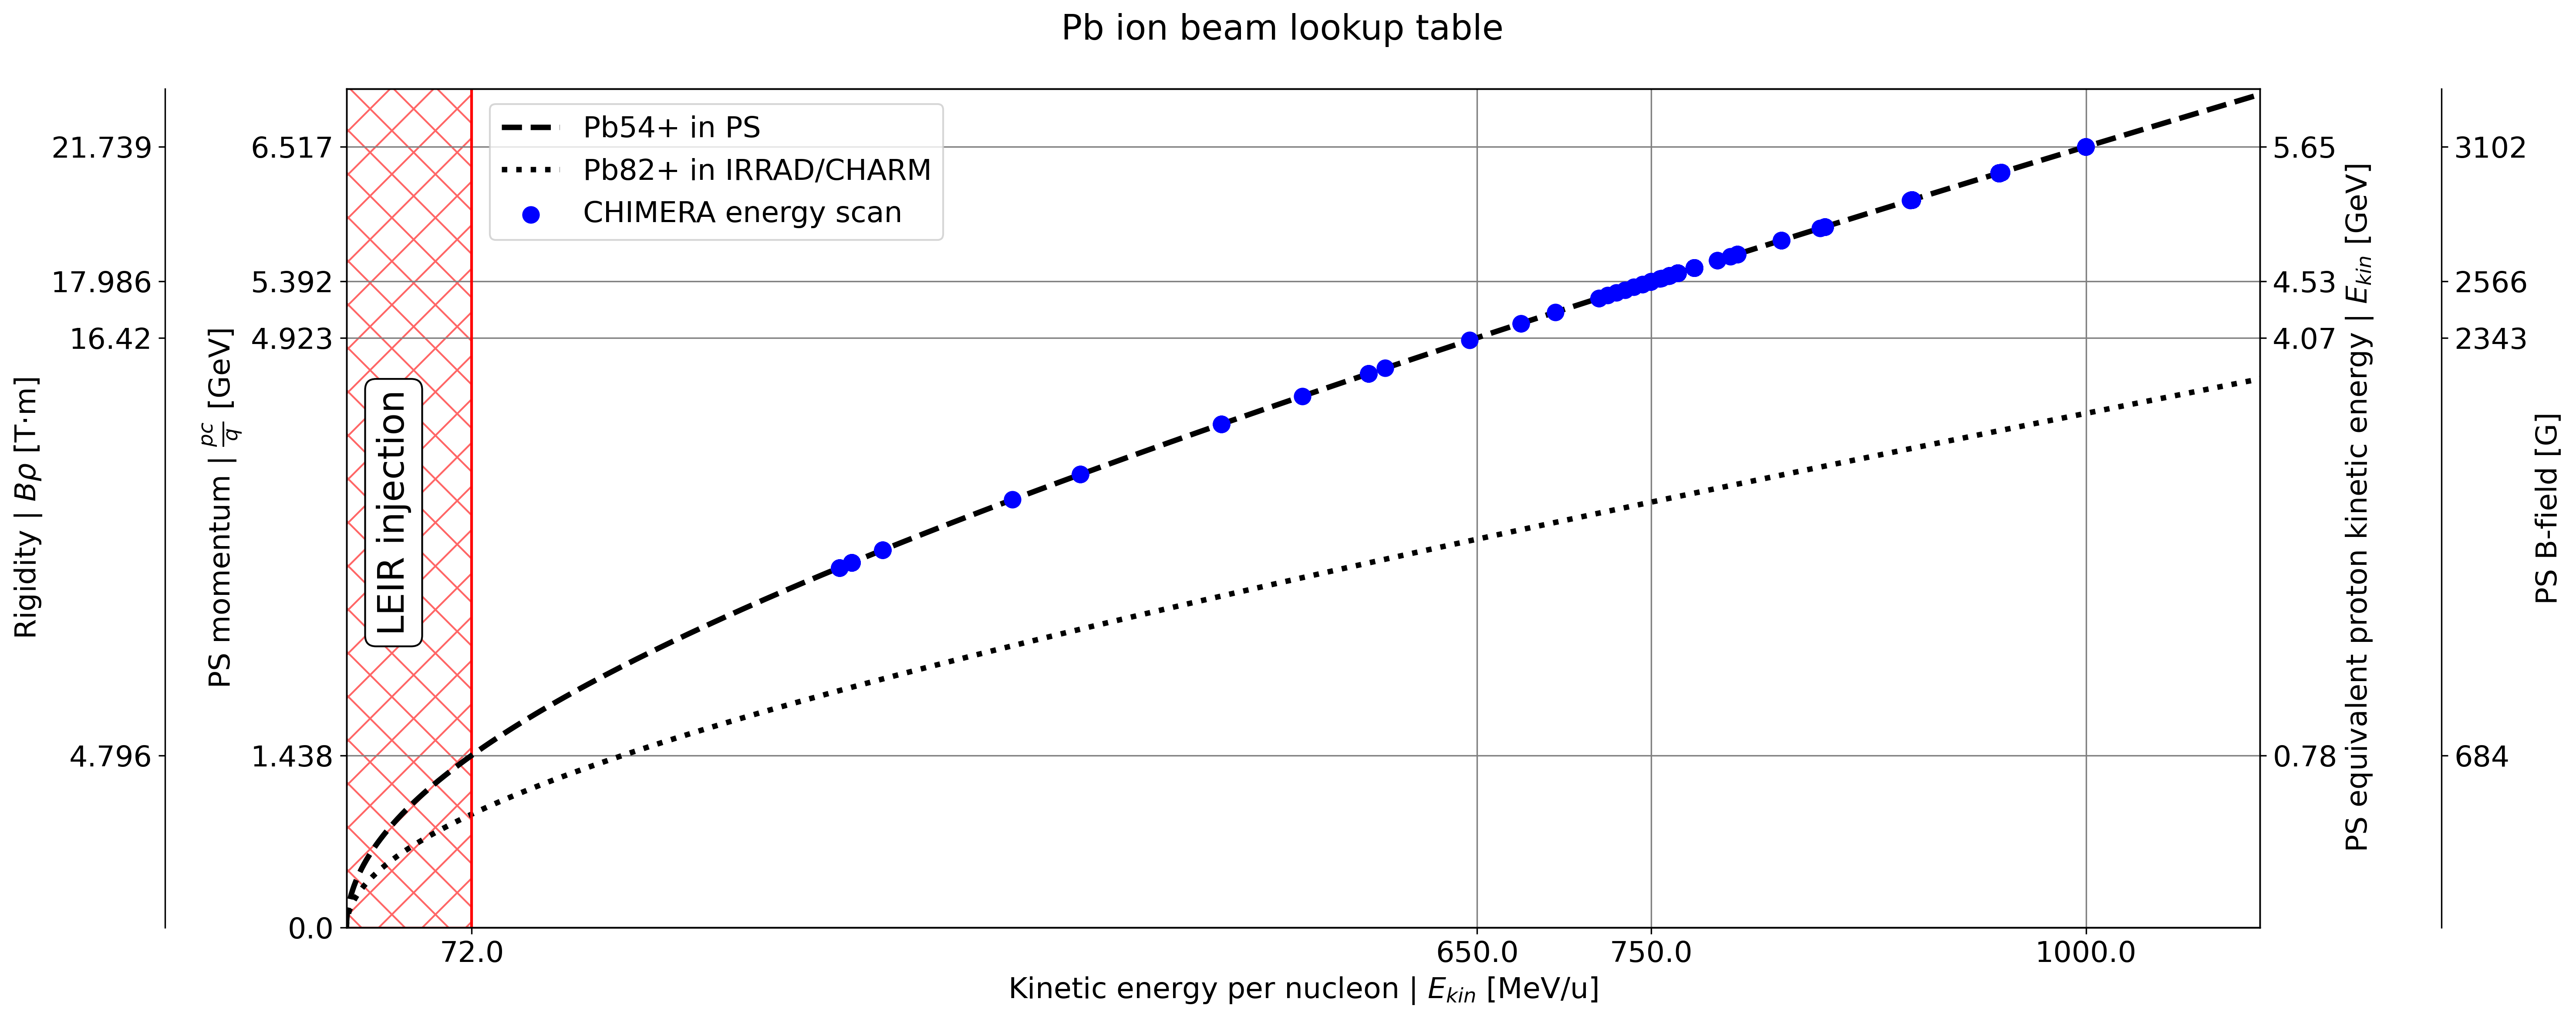
\includegraphics[width=1.0\textwidth]{images/PS_BEAM_ENERGY/kinetic_energy_lookup_chimera.png}
\caption{Lookup table for the lead ion beam flat-top in the Proton Synchrotron (PS). The magnetic field required for acceleration to three different energies (1000, 750, and 650 MeV/$u$) as well as energy scan measurements to the East Dump is shown.}
\label{fig:lookup table}
\end{figure}

\begin{table}[!htbp]
\centering
\begin{threeparttable}
\label{tab:KE_table}
\begin{tabular}{@{}m{1.6cm}m{1.6cm}m{2.8cm}m{2.8cm}m{4cm}@{}}
\toprule
$E^{PS}_{kin}$ {[}MeV/$u${]} & $E^{DUT}_{kin}$\tnote{$\dagger$} [MeV/$u$] & $LET^{PS}$\tnote{$\dagger$} [MeV$\cdot$~cm$^2$/mg] & $LET^{DUT}$\tnote{$\dagger$} [MeV$\cdot$~cm$^2$/mg] & USER \\ \midrule
1000 & 600 & 11 & 13 & CPS.USER.EAST4 \\
750 & 300 & 12 & 18 & CPS.USER.EAST3 \\
650 & 150 & 13 & 27 & CPS.USER.MD5 \\ \bottomrule
\end{tabular}
\begin{tablenotes}
\item[$\dagger$] FLUKA simulation.
\end{tablenotes}
\caption{Table showing the kinetic energy and LETs used during the ESA November 2022 run at flat-top in the PS and at the DUT. The term 'USER' refers to the settings the PS is loaded with. A USER profile saves all magnet strengths, which can be easily accessed and applied to the PS when that particular USER is called, similar to a preset configuration.}
\end{threeparttable}
\end{table}


Figure \ref{fig:bfield} illustrates the magnetic field profile of the main dipoles in the Proton Synchrotron (PS) produced by the main magnet power supply (POPS). The profile includes two distinct regions - the injection plateau where ions are injected from LEIR, and the flat-top extraction plateau where ions have achieved maximum energy and are ready for extraction. Note that the spike at the end, which was introduced to overcome certain limitations of POPS, is irrelevant to the extraction process and can be disregarded.

\begin{figure}[!htb]
\centering
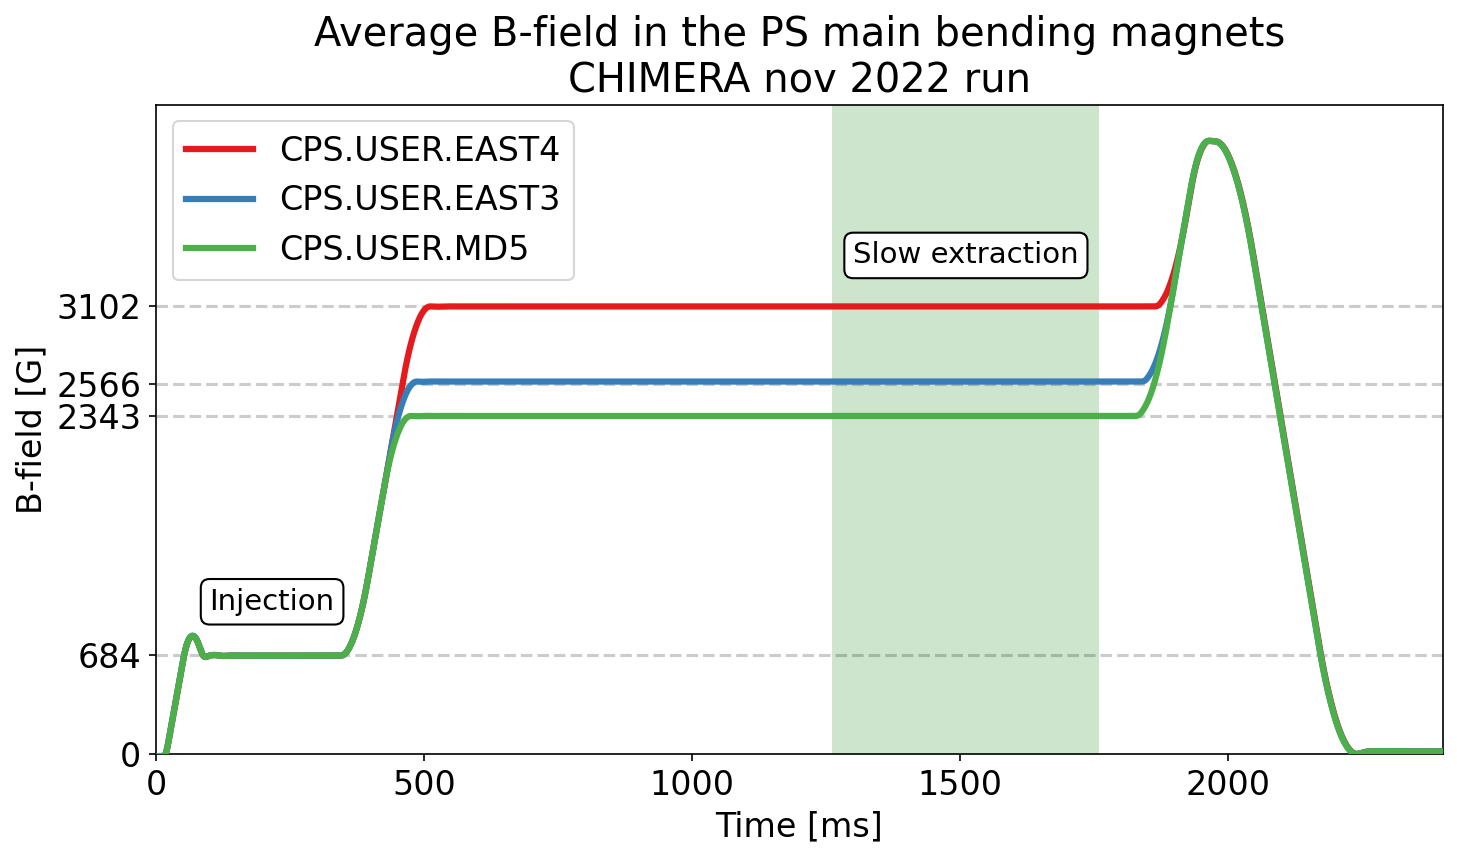
\includegraphics[width=0.6\textwidth]{images/PS_BEAM_ENERGY/average_b_field_chimera.png}
\caption{CHIMERA's magnetic field at different energies, with injection plateau at 684 G and extraction plateau at varying B-field strengths corresponding to different energy levels.}
\label{fig:bfield}
\end{figure}

During the CHIMERA ion run in November, the experiment lasted for 5 days, from the afternoon of Wednesday 23 November to the  morning of Monday 28 November. The energies used during the run were 1000, 750, and 650 MeV/$u$ and were used for almost the same amount of time. The 650 MeV/$u$ beam was used for 36\% of the time, the 750 MeV/$u$ beam was used for 28\%, and the 1000 MeV/$u$ beam was used for 35\%. The run was divided into specific tasks and timeframes, see Fig. \ref{fig:timestamp_energies}. Wednesday and Thursday were used for beam preparation, Friday and Saturday were devoted to ESA's experiments, and Sunday was used for backup or for additional machine development. During the first few hours of the beam time, the focus was on characterizing the three energies and varying the intensity using the standard beam instruments. The next few hours were dedicated to testing all four DUTs sequentially for all energies, followed by a run overnight to accumulate statistics on the Renesas memory \cite{noauthor_rmlv0816bgsa_nodate}. On Thursday morning, the team changed the degrader thickness twice. Friday and if needed part of Saturday were dedicated to ESA's experiment. The rest of Saturday night and Sunday were left for backup and for optics measurements.

\begin{figure}[!htb]
\centering
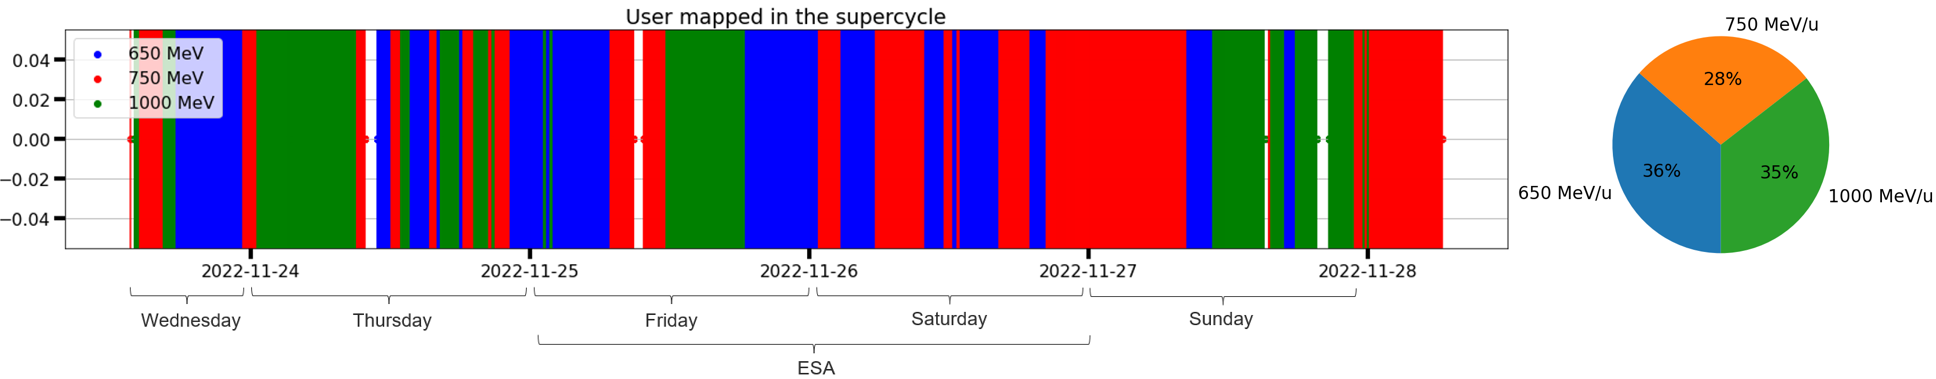
\includegraphics[width=1.0\textwidth]{images/PS_BEAM_ENERGY/user_mapping_timestamp.png}
\caption{Timestamps of beam energies: the plot displays the time stamps associated with different beam energies used during the November run.}
\label{fig:timestamp_energies}
\end{figure}

Following the ESA run, an automatic script was used to ramp the beam energy for further development purposes. A dedicated energy scan was conducted on the diode using 5 different beam energies, ranging from 775 MeV/$u$ to 900 MeV/$u$. A separate experiment was carried out to measure the lowest beam energy that could be recorded at the East Dump, which was found to be 283 MeV/$u$. The main limitation was that the bending magnet to the dump is not scaled with momentum, and hand corrections were needed to propagate the beam to the dump (which could be scaled and set by a script), as well as the beam spot on the BTV being large and weak at this energy, which made observation difficult. Lower energies could be tried out in the future.

\begin{figure}[!htb]
    \centering
    \begin{minipage}{0.45\textwidth}
        \centering
        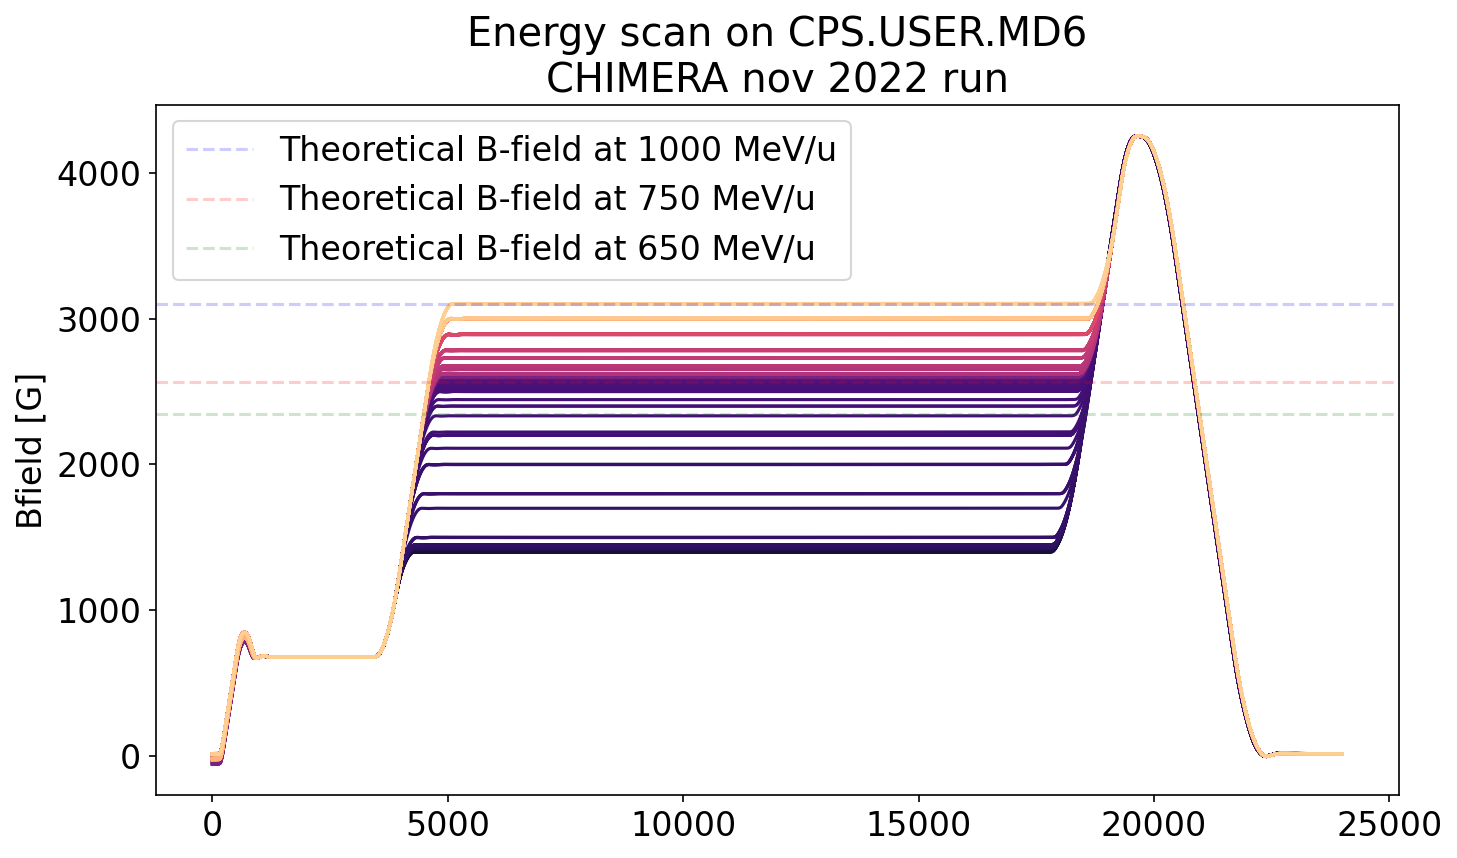
\includegraphics[width=1.0\textwidth]{images/PS_BEAM_ENERGY/energy_scan_chimera 1.png}
        \caption{Plot of the B-field showing different flat-tops during an energy scan.}
        \label{fig:energy_scan}
    \end{minipage}\hfill
    \begin{minipage}{0.45\textwidth}
        \centering
        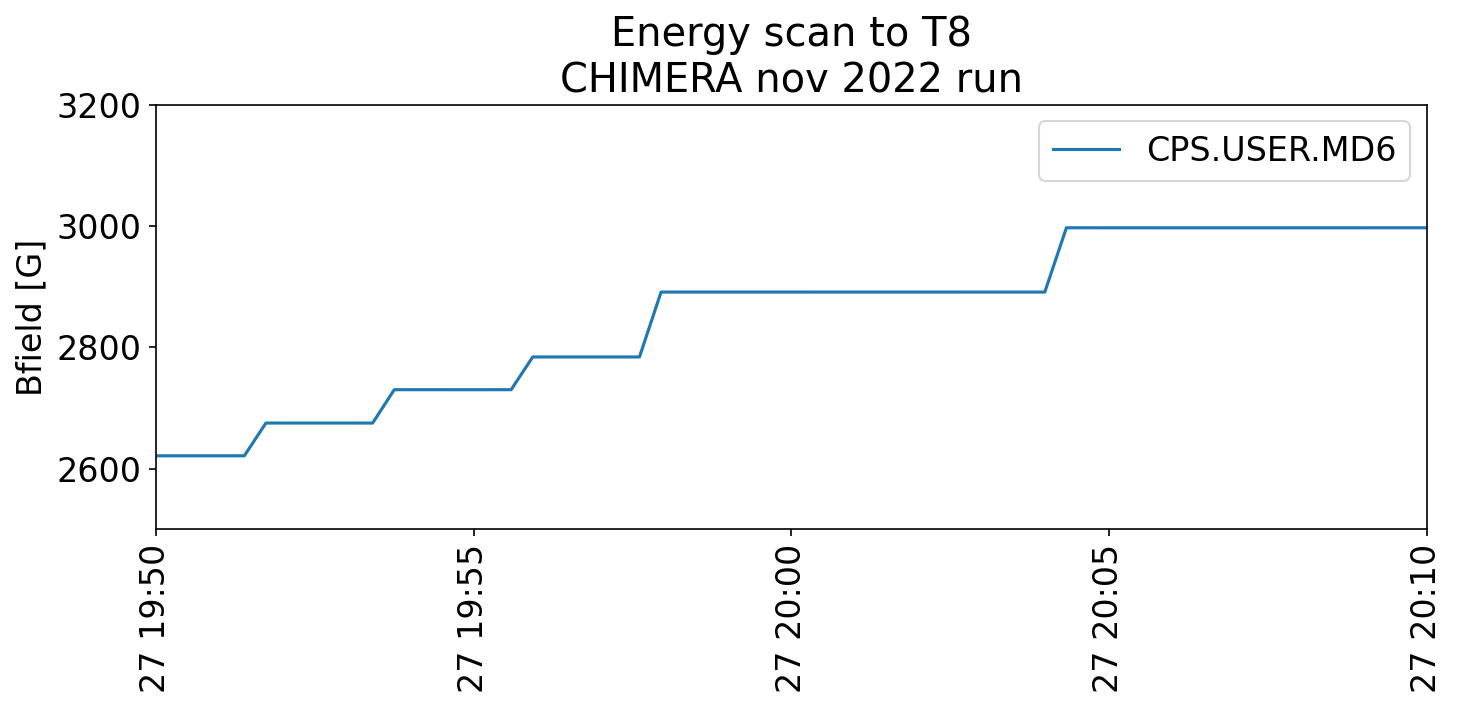
\includegraphics[width=1.0\textwidth]{images/PS_BEAM_ENERGY/energy_scan_timestamp_chimera 1.png} 
        \caption{Energy scan with timestamp.}
        \label{fig:energy_scan_timestamp}
    \end{minipage}
\end{figure}


%%%%%%%%%%%%%%%%%%%%%%%%%%%%%%%%
%%%%%% Conclusion %%%%%%%%%%%%%%
%%%%%%%%%%%%%%%%%%%%%%%%%%%%%%%%

\section{Conclusion}

 The primary beam energy determines the Linear Energy Transfer (LET) of the incident particles, which affects the type and amount of radiation-induced effects on the electronic components being tested. Controlling the primary beam energy is therefore crucial for radiation testing of electronic components. In the context of the CHIMERA project at CERN, the primary beam energy was varied by scaling the magnetic field in the Proton Synchrotron (PS) during acceleration and transport and with the PFWs removed from operation. The PS's magnet strengths were adjusted by a makerule that computed the magnetic field required for a given beam energy, allowing automatic scaling of magnets in F61 and the T8 transfer line. The November 2022 run of CHIMERA demonstrated the effectiveness of the system, with the successful testing of four Device Under Test (DUT) setups, a degrader scan, and measurements of the three beam energies. The system provides an important solution for controlling primary beam energy and exploring a wide range of LET values.

\bibliography{references}
\bibliographystyle{IEEEtran}

\end{document}
